\section{State of the Art}
% presentation de la dynamique et hypothèse

\begin{frame}{State of the Art}
\framesubtitle{The dynamics of the system}

\begin{columns}
\column{4cm}
\begin{cadre}

\begin{center}
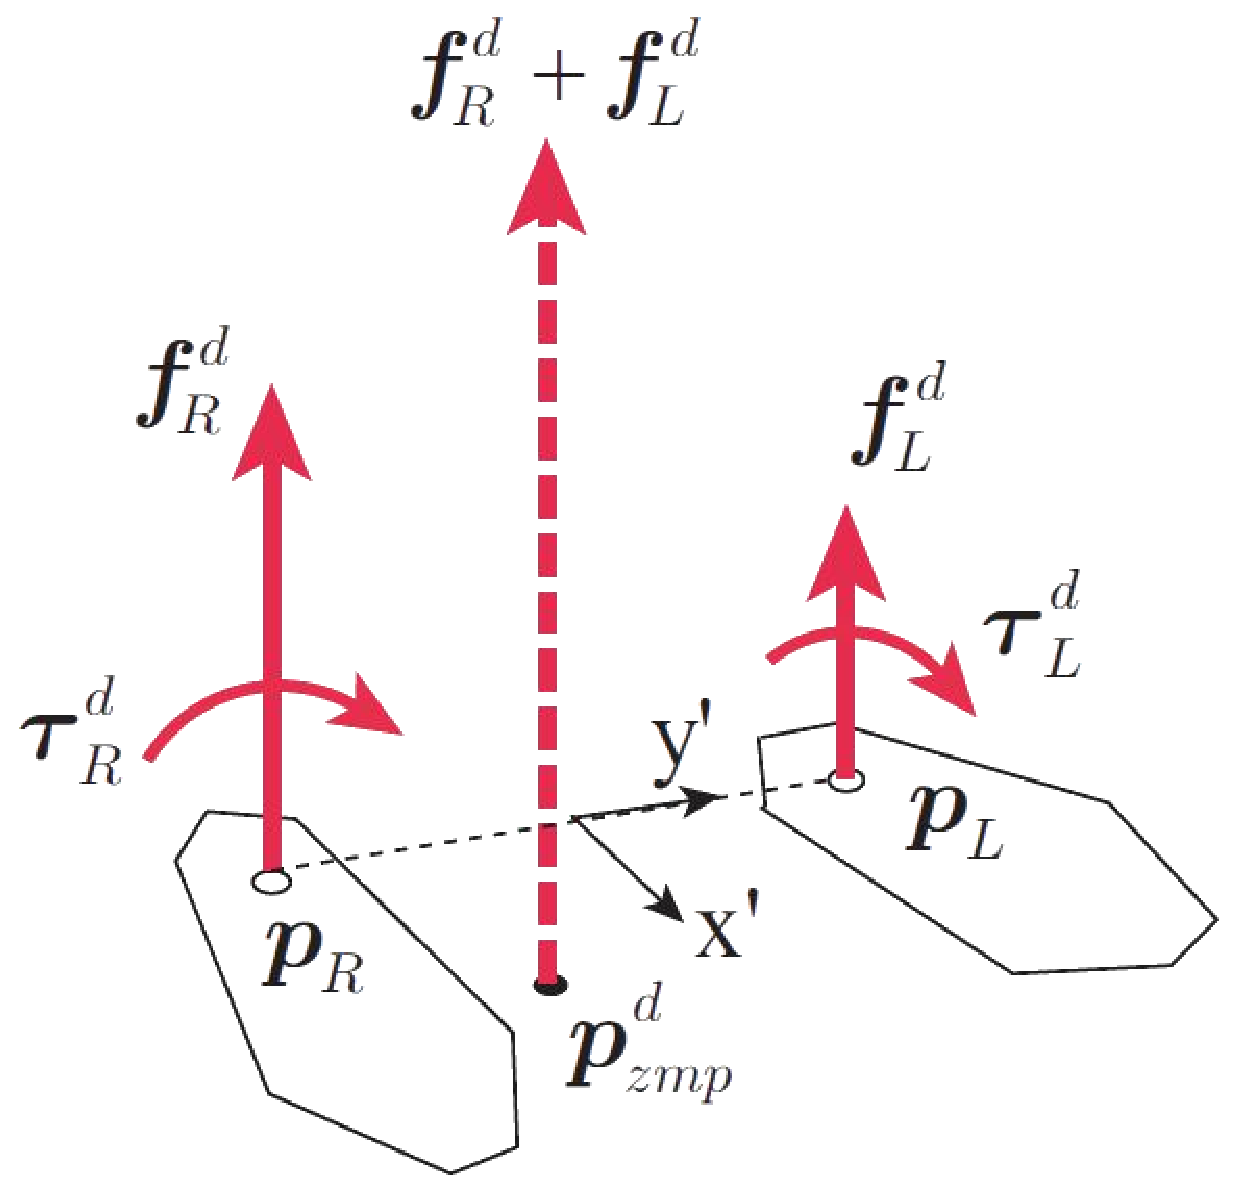
\includegraphics[scale=0.2]{forces-ground}
\end{center}

\end{cadre}

\column{6cm}    
\begin{cadre}

\begin{equation*}
\left\lbrace
\begin{aligned}
&m\,( \mathbf{ \ddot{c} } - \mathbf{g}) = \sum_{i} \mathbf{R} _{i} \mathbf{f} _{i}   \\
&m \,\mathbf{c} \times ( \mathbf {\ddot{c}} - \mathbf{g} ) = \mathbf{p}^d_{zmp} \times \sum_{i} \mathbf{R} _{i} \mathbf{f} _{i}\\
\end{aligned}
\right.
\label{eq:underactuated_dynamics}
\end{equation*}

${\bf p}_{zmp}^d$ : zero momentum point.\\

Stability criteria : \\
{\color{black!20!red} cop inside the convex support polygon}\\
$ \rightarrow {\bf p}^d_{zmp} = {\bf p}^d_{cop}
\; \text{(center of pressure)} $
\end{cadre}
\end{columns}

\end{frame}


\begin{frame}{State of the Art}

\begin{table}
\footnotesize
\begin{tabularx}{340pt}{ | X | X | X | X | }
\hline
Type of solution & Advantages & Disadvantages & Famous Authors \\
\hline \hline
Analytical Solution & very fast to compute & not flexible & Morisawa(ICRA 2007) \\
\hline
Numerical Solution & complex to compute & flexible & Kajita(ICRA 2003), Herdt(Advanced Robotics 2010) \\
\hline
\end{tabularx}
\end{table}

Some videos of walking humanoid robots :\\
\begin{itemize}
  \item \href{https://www.youtube.com/watch?v=diaZFIUBMBQ}
    {\color{black!20!red} Shaft from the University of Tokyo}
  \item \href{https://www.youtube.com/watch?v=SD6Okylclb8}
    {\color{black!20!red} Atlas from Boston Dynamics}
\end{itemize}


\end{frame}
